\documentclass{article}
\usepackage{enumitem}
\usepackage[cachedir=minted_cache]{minted}
\usepackage{graphicx}
\graphicspath{ {./img/} }
\usepackage[margin=1in]{geometry} %used to set the margins
\setcounter{secnumdepth}{0} %used to get rid of section numbers
\title{Lab 6\\ Sets and Union/Find Structures}
\author{Michael Morikawa \& James Daza}
\date{\today}


\begin{document}
\maketitle
\section{Lab Questions}
\begin{enumerate}[label=\textbf{Question \arabic*}]
    \item Describe the template method pattern.\\
          \textbf{
              It is a design pattern that uses a generic way to solve a problem, and then redefined certain
              steps of that process to fit the specifics of the problam that you are trying to solve.
          }
    \item What are some applications for the find/union partition structures?\\
          \textbf{
              Some applications for this data structure is to keep track of connected components of a graph and is also used in other
              graph related algorithms.
          }


\end{enumerate}

\section{Source Code}
\subsection{Merge.hpp}
\inputminted{c++}{../include/Merge.hpp}
\subsection{main.cpp}
\inputminted{c++}{../src/main.cpp}

\section{Output}
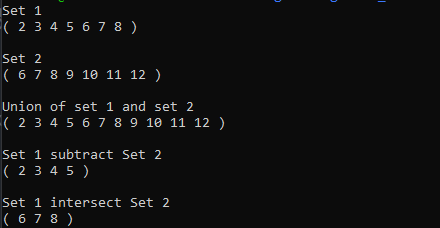
\includegraphics[]{output.png}

\end{document}